\documentclass[a4paper,oneside,12pt]{article}
\usepackage[portuguese]{babel}
\usepackage{graphicx}
\usepackage{listings}
\usepackage{indentfirst}
\usepackage{fontspec}
\usepackage{hyperref}

\usepackage{xcolor}

\definecolor{codegreen}{rgb}{0,0.6,0}
\definecolor{codegray}{rgb}{0.5,0.5,0.5}
\definecolor{codepurple}{rgb}{0.58,0,0.82}
\definecolor{backcolour}{rgb}{0.95,0.95,0.92}
\definecolor{bg}{rgb}{0.8, 0.8, 0.8}

\lstdefinestyle{mystyle}{
    backgroundcolor=\color{backcolour},   
    commentstyle=\color{codegreen},
    keywordstyle=\color{magenta},
    numberstyle=\tiny\color{codegray},
    stringstyle=\color{codepurple},
    basicstyle=\ttfamily\footnotesize,
    breakatwhitespace=false,         
    breaklines=true,                 
    captionpos=b,                    
    keepspaces=true,                 
    numbers=left,                    
    numbersep=5pt,                  
    showspaces=false,                
    showstringspaces=false,
    showtabs=false,                  
    tabsize=2
}

\lstset{style=mystyle}

\newcommand{\mybox}[1]{
    \colorbox{backcolour}{\textbf{#1}}
}

\linespread{1.5}
\setmainfont{Times New Roman}

\title{Metaballs com LÖVE}
\author{Canoi Gomes}
\date{22 de Janeiro de 2017}

\begin{document}

\maketitle
\newpage

\tableofcontents
\newpage

\section{Introdução}

Nesse tutorial pretendo mostrar como que é possível criar o efeito de metaballs usando a framework LÖVE. Não é nada de outro mundo, é um efeito que você pode reproduzir em diferentes engines, e acredito que sem muita dificuldade.

\subsection{Baixando a LÖVE}

Entre no site \url{https://love2d.org} e baixe a versão para o seu sistema operacional. No Linux a maioria das distribuições devem ter presentes a framework em seu repositório, algumas talvez só estejam desatualizadas. Para o Windows é preciso baixar do site mesmo, e também adicionar a pasta de instalação nas variáveis do sistema.

\subsection{O que são metaballs?}

Bom, simplificando bastante, metaball é o nome dado para um efeito na computação gráfica onde os objetos parecem conseguir se mesclar um com o outro de maneira homogênea.

Algo tipo isso aqui:

\begin{figure}[h]
    \centering
    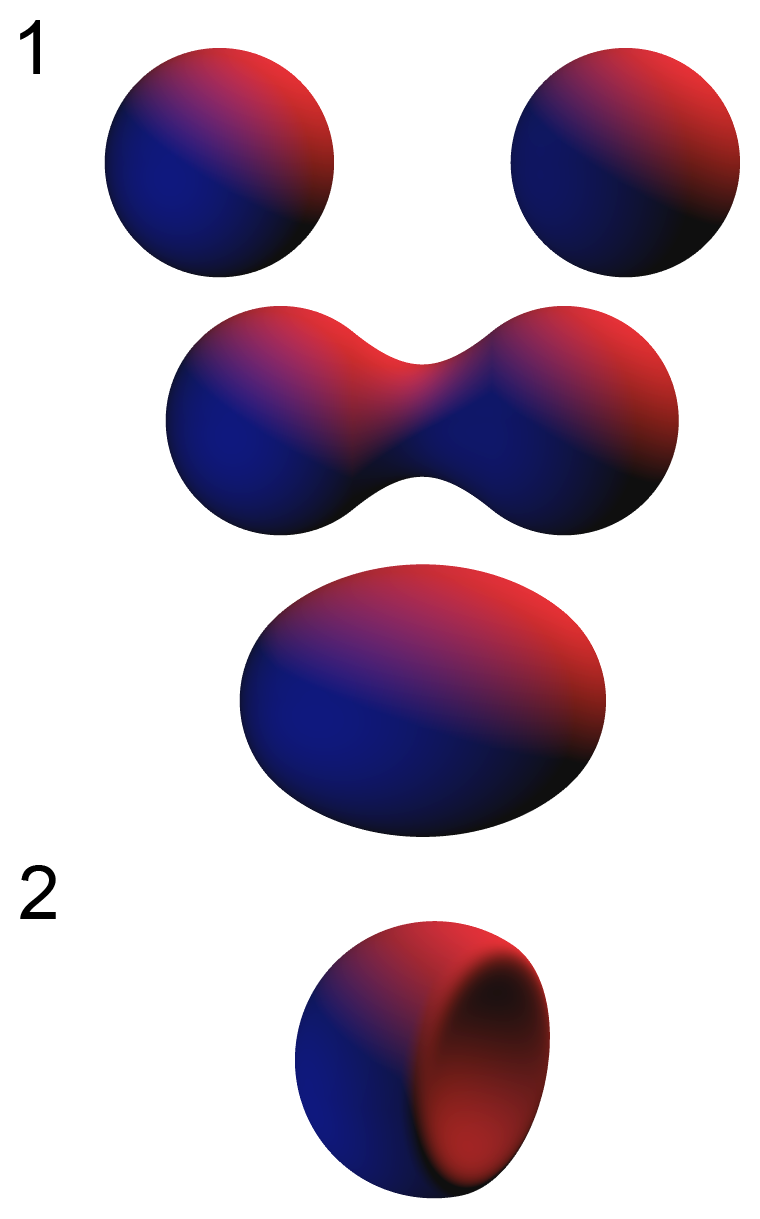
\includegraphics[width=0.5\linewidth]{media/metaballs.png}
\end{figure}
\break

\section{Começando o Código}

Para criar um programinha que rode em lua é bem simples, depois de ter baixado é só criar o diretório do seu projeto e criar um arquivo \textbf{main.lua} dentro dele. Entrando nesse diretório pelo terminal e rodando o comando \textbf{love .} já deve ser o suficiente para rodar seu projeto. O conteúdo do documento precisa ser o seguinte:

\begin{lstlisting}[language={[5.2]Lua}]
function love.load()
end

function love.update(dt)
end

function love.draw()
end
\end{lstlisting}

Que é a estrutura básica do código LÖVE. A imagem que vou utilizar para a metaball será essa aqui:

\begin{figure}[h]
    \centering
    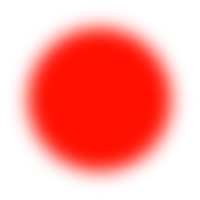
\includegraphics[width=.2\linewidth]{media/metaball.png}
\end{figure}

E agora vamos começar a escrever a lógica. Primeiramente vou criar uma tabela para guardar todas as minhas metaballs e vou também criar um construtor pra facilitar minha vida.

\begin{lstlisting}[language={[5.2]Lua}]
metaballs = {}
function createMetaball(x, y)
  local metaball = {
    x = x or 0,
    y = y or 0,
    vx = 0,
    vy = 0,
    size = 1
  }
  return metaball
end

function love.load()
end

function love.update(dt)
end

function love.draw()
end
\end{lstlisting}

As propriedades da metaball são as seguintes:

\begin{itemize}
    \item \textbf{x e y}: As posições
    \item \textbf{vx e vy}: A velocidade que a bola irá se mexer em cada eixo
    \item \textbf{size}: Tamanho da metaball
\end{itemize}

Agora vamos carregar nossa imagem para poder usar, e também vamos criar um canvas para que possamos desenhar nele, e posteriormente aplicar o efeito que dará vida a nossas metaballs.

\begin{lstlisting}[language={[5.2]Lua}]
function love.load()
    metaball_image = love.graphics.newImage("metaball.png")
    canvas = love.graphics.newCanvas(800, 600)
end
\end{lstlisting}

E com isso eu posso começar a desenhar algo na tela. Vou desenhar uma metaball na posição do meu mouse, e também vou começar a aplicar o canvas na tela.

\begin{lstlisting}[language={[5.2]Lua}]
function love.update(dt)
    mx, my = love.mouse.getPosition()
end

function love.draw()
    love.graphics.setCanvas(canvas)
    love.graphics.clear(0,0,0,0)
    love.graphics.draw(metaball_image, mx, my, 0, 1, 1, 100, 100) -- ajusta o offset para desenhar o centro da imagem na posição do mouse
    for i,v in ipairs(metaballs) do
        love.graphics.draw(metaball_image, v.x, v.y, 0, v.size, v.size)
    end
    love.graphics.setCanvas()
    love.graphics.draw(canvas)
end
\end{lstlisting}

Agora vamos criar o shader para aplicarmos no canvas. O nome do efeito se chama \textbf{Alpha Threshold}, é um shader que vai limitar o alpha da nossa imagem até um certo valor (que pode ser personalizado por nós).

\begin{lstlisting}[language=C]
vec4 effect(vec4 color, Image texture, vec2 tex_coord, vec2 screen_coord) { 
    vec4 pixel = Texel(texture, tex_coord); 
    if (pixel.a <= threshold)
        pixel.a = 0.0;
    return pixel * color;
}
\end{lstlisting}

Onde \textbf{threshold} é exatamente esse valor limite que podemos definir para o alpha, e o alpha que for menor que esse limite será truncado para zero. Para criar esse shader na LÖVE eu posso fazer o seguinte:

\begin{lstlisting}[language={[5.2]Lua}]
function love.load()
metaball_image = love.graphics.newImage("metaball.png")
    canvas = love.graphics.newCanvas(800, 600)
    shadersrc = [[ 
    vec4 effect(vec4 color, Image texture, vec2 tex_coord, vec2 screen_coord) { 
        vec4 pixel = Texel(texture, tex_coord); 
        if (pixel.a <= 0.6)
        pixel.a = 0.0;
        return pixel * color;
    }
    ]]
    shader = love.graphics.newShader(shadersrc)
end

function love.update(dt)
    mx, my = love.mouse.getPosition()
end

function love.draw()
    love.graphics.setCanvas(canvas)
    love.graphics.clear(0,0,0,0)
    love.graphics.draw(metaball_image, mx, my, 0, 1, 1, 100, 100)
    for i,v in ipairs(metaballs) do
        love.graphics.draw(metaball_image, v.x, v.y, 0, v.size, v.size)
    end
    love.graphics.setCanvas()
    love.graphics.setShader(shader)
    love.graphics.draw(canvas)
    love.graphics.setShader()
end
\end{lstlisting}

Isso já é o suficiente para o nosso efeito estar funcionando, porém para visualizar precisamos criar outras metaballs. Pra isso vou fazer uma lógica bem simples para adicionar uma nova bola na minha tabela toda vez que eu clicar com o mouse. Ficaria assim:

\begin{lstlisting}[language={[5.2]Lua}]
local time = 0
function love.update(dt)
    mx, my = love.mouse.getPosition()
    time = time + dt
    if love.mouse.isDown(1) and time >= 0.4 then
        time = 0
        local meta = createMetaball(mx, my)
        meta.vx = love.math.random(-200, 200)
        meta.vy = love.math.random(-200, 200)
        meta.size = love.math.random() + 0.1
        table.insert(metaballs, meta)
    end
end
\end{lstlisting}

Vou adicionar também um update para fazer essas bolas se mexerem:

\begin{lstlisting}[language={[5.2]Lua}]
function createMetaball(x, y)
  local metaball = {
    x = x or 0,
    y = y or 0,
    vx = 0,
    vy = 0,
    size = 1,
    update = function(self, dt)
      self.x = self.x + (self.vx * dt) 
      self.y = self.y + (self.vy * dt) 
      if self.x >= screen_width or self.x <= 0 then 
        self.vx = self.vx * -1 
      end 
      if self.y >= screen_height or self.y <=0 then
        self.vy = self.vy * -1
      end
    end
  }
  return metaball
end
\end{lstlisting}

E no update:

\begin{lstlisting}[language={[5.2]Lua}]
local time = 0
function love.update(dt)
    mx, my = love.mouse.getPosition()
    time = time + dt
    if love.mouse.isDown(1) and time >= 0.4 then
        time = 0
        local meta = createMetaball(mx, my)
        meta.vx = love.math.random(-200, 200)
        meta.vy = love.math.random(-200, 200)
        meta.size = love.math.random() + 0.1
        table.insert(metaballs, meta)
    end
    for i,v in ipairs(metaballs) do
        v:update(dt)
    end
end
\end{lstlisting}

\end{document}